
\usetikzlibrary{arrows.meta,calc,shapes,decorations.pathreplacing,patterns}
\providecommand{\computer}{%
    
\includegraphics[width=1cm]{../common/Noun_project_216.pdf}
}
\providecommand{\switch}{%
    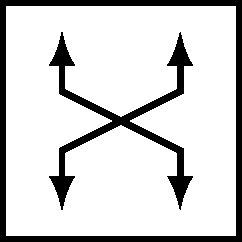
\includegraphics[width=0.9cm]{../common/fig-switch.pdf}
}
\providecommand{\router}{%
    
\includegraphics[width=0.9cm]{../common/fig-router.pdf}
}


\begin{frame}{long links}
\begin{tikzpicture}
\tikzset{
    computer/.style={inner sep=0mm,outer sep=0mm,execute at begin node={\computer}},
    switch/.style={inner sep=0mm,outer sep=0mm,execute at begin node={\switch}},
    router/.style={inner sep=-1mm,outer sep=0mm,execute at begin node={\router},circle},
    connect/.style={draw,line width=0.5mm,Latex-Latex},
    connect big/.style={draw,line width=1mm,Latex-Latex},
}
\node[computer] (A) at (0, 2){};
\node[computer] (B) at (13, 0){};
\node[router] (r1) at (5, 0){};
\node[router] (r2) at (10, 0){};
\node[computer] (C) at (-1, -4){};
\node[computer] (D) at (12, -2){};
\foreach \x/\y in {A/r1,r1/r2,r2/B,r2/D} {
    \draw[connect big] (\x) -- (\y);
}
\draw[connect big] (C) -- (r1)
    node[-,sloped,midway,pin={long link},every pin edge/.style={-}] {};
\begin{visibleenv}<2>
\foreach \x/\y in {A.east/r1.west,r1.east/r2.west,r2.east/B.west} {
    \draw[-Latex,blue,line width=.7mm] ([yshift=-3mm]\x) -- ([yshift=-3mm]\y);
}
\foreach \x/\y in {C.north east/r1.south west,r1.east/r2.west,r2/D} {
    \draw[-Latex,red,dotted,line width=.7mm] ([yshift=3mm]\x) -- ([yshift=3mm]\y);
}
\end{visibleenv}
\end{tikzpicture}
\end{frame}

\begin{frame}{exercise: window size?}
    \begin{itemize}
    \item flow 1: 500 packets/sec, 50 ms round trip
    \item flow 2: 500 packets/sec, 100 ms round trip
    \vspace{.5cm}
    \item exercise: what window size achieves this for each flow?
        \begin{itemize}
        \item<2-> 1: window size 25; 2: window size 50
        \end{itemize}
    \end{itemize}
\end{frame}

\begin{frame}{revisiting additive increase}
    \begin{itemize}
    \item TCP: add +1 to window size each round trip time
    \item flow 1: window 25+1 $\rightarrow$ 26 pkt/50 ms = 520 pkt/sec
    \item flow 2: window 50+1 $\rightarrow$ 51 pkt/100 ms = 510 pkt/sec
    \end{itemize}
\begin{tikzpicture}
\tikzset{
    axis/.style={
        draw,ultra thick,-Latex
    },
    normal mark/.style={
        fill=black,
    },
    normal adjust/.style={
        line width=.5mm,draw=black!50!red,-Latex,
    },
}
\begin{scope}[x=.8cm,y=.8cm] 
    \path[fill=red!10] (5.5, 0) -- (5.0, 0) -- (0, 5) -- (0, 5.5) -- (5.5, 5.5) -- cycle;
    \path[axis] (0, 0) -- (5.5, 0)
        node[midway,below] {flow 1 bandwidth};
    \path[axis] (0, 0) -- (0, 5.5)
        node[midway,left,align=right] {flow 2\\bandwidth};
    \path[draw,dashed,very thick] (5, 0) -- (0, 5);

    \begin{visibleenv}<2>
        \path[draw,dotted,very thick] (0, 0) -- (3.333 * 1.5, 1.667 * 1.5);
        \path[draw,dotted,very thick] (2, 2) -- ++(3.333 * 1, 1.667 * 1);
        \path[draw,dotted,very thick] (2, 2) -- ++(-3.333 * 0.7, -1.667 * 0.7);
    \end{visibleenv}

    \path[normal adjust] (2, 2) -- ++(1, .5);
    \path[normal mark] (2, 2) circle (1mm);
    \path[dotted,-Latex,line width=.5mm,draw=black!50] (2,2) -- ++ (1, 1);
    \begin{visibleenv}<1>
    \node[align=left,anchor=west] at (6, 2.5) {
        flow 1 increases faster \\
        than flow 2 increases \\
        not 45-degree angle anymore
    };
    \end{visibleenv}
    \begin{visibleenv}<2>
        \path[fill=red] (3.333, 1.667) circle (2mm);
        \path[fill=black] (3.333, 1.667) circle (1mm);
        \node[align=left,anchor=west] at (6, 2.5) {
            in equilibrium \\
            flow 1 gets more bandwidth
        };
        \end{visibleenv}
\end{scope}
\end{tikzpicture}
\end{frame}
